\documentclass[11pt]{article}
\usepackage[margin=1in]{geometry}
\usepackage{graphicx}
\usepackage{microtype}
\usepackage{verbatim}
\usepackage{amsmath}
\usepackage{nicefrac}
\usepackage[colorlinks=false, hidelinks]{hyperref}
\usepackage{caption}
\usepackage{subcaption}
\usepackage{listings}
\usepackage{harmony}
\usepackage{wasysym}
\usepackage{color}

\definecolor{mygray}{rgb}{.9,.9,.9}
\lstset{ %
	breaklines=true
	language=[x86masm]Assembler,
  	backgroundcolor=\color{white},   % choose the background color; you must add \usepackage{color} or \usepackage{xcolor}
	numberstyle=\small\color{mygray}, % the style that is used for the line-numbers
	numbers=none,                    % where to put the line-numbers; possible values are (none, left, right)
}

\begin{document}

\title{Switch Bounce \& Catch the Clown Game\\Embedded System Design, Lab 6}
\date{November 5, 2015}
\author{Ben Lorenzetti}
\maketitle

\tableofcontents

\clearpage

\section{Objectives and Problem Description}

\subsection{Part 1: Does the Switch Bounce?}
\label{switch-debounce-problem-specs}

\subsection{Part 2: Catch the Clown!}
\label{catch-the-clown-problem-specs}

Build a game for testing reaction times with an 8 LED rotating display,
a pushbutton trigger, and a knob for adjusting the speed/difficulty.
If the player presses the trigger in sync with
the LED display, then the display stops rotating to indicate victory.
The specifications can be summarized in the four points below:
\begin{enumerate}
\item For an 8 LED display, one LED should be illuminated at a time and
the illuminated position should rotate right one digit every period.
\item The period should be adjustable on the fly with the rotatry potentiometer knob.
\item If the user triggers the switch while the topmost (most significant bit) 
LED is illuminated, then the LED display should stop rotating
until the switch is released. The LED rotation loop should also continue--\mbox{including
through the topmost state}--if the switch is active but was triggered
during the wrong state.
\item The pushbutton switch should be debounced based on the results from
part 1.
\end{enumerate}

\section{Procedure}

\subsection{Switch Bounce Background}

Mechanical switches do not always produce clean, step function electrical signals.
Instead, when a switch is thrown, the electric signal often `bounces' several times
before settling at the active level. This is caused by electric arcing and breaking
as the contacts near one other and from mechanical vibrations of contacts from the
throwing force.

Bouncing can cause problems if the device's function depends on the number of times
a switch is thrown. For example, if you keyboard bounced, you would find yourself
typing repeat letters and unpredictable backspacing. Traditionally switches were
`debounced' with low pass filters in hardware, but with fast microcontrollers
debouncing can be done in software to reduce hardware costs.
\hyperref[io-circuit-diagram]{Figure \ref{io-circuit-diagram}} shows how PIC did this
with their PIC16F887 44--pin demo board.

\begin{figure}
\centering
	\begin{subfigure}[b]{.4\textwidth}
		\centering
		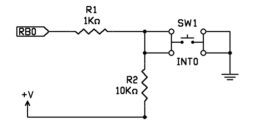
\includegraphics[width=\textwidth]{Figures/demo-board-pushbutton-circuit.pdf}
		\caption[]%
		{{PIC16F887 Demo Board Schematic: \emph{pushbutton SW1 is unfiltered and requires software debouncing.}}}
	\end{subfigure}
	\quad
	\begin{subfigure}[b]{0.5\textwidth}
		\centering
		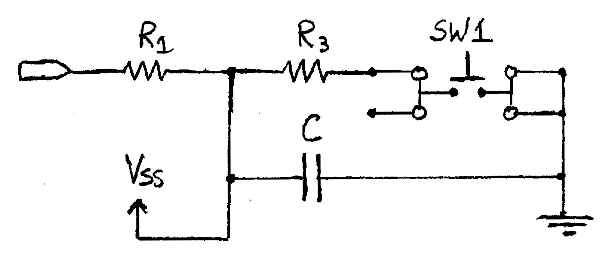
\includegraphics[width=\textwidth]{Figures/filtered-pushbutton-circuit.pdf}
		\caption[]%
		{{\small A Hardware Debounced Pushbutton: \emph{\mbox{$R_{3}$ and $C$} form a low pass filter.}}}
	\end{subfigure}	
	\caption{Hardware vs Software Debouncing for Mechanical Switches}
	\label{io-circuit-diagram}
\end{figure}

\subsection{Part 1: Debouncing \texttt{SW1}}

\subsection{Part 2: Catch the Clown Game}

\section{Expected Results}

\subsection{Debounce Time}

\begin{figure}
	\centering
	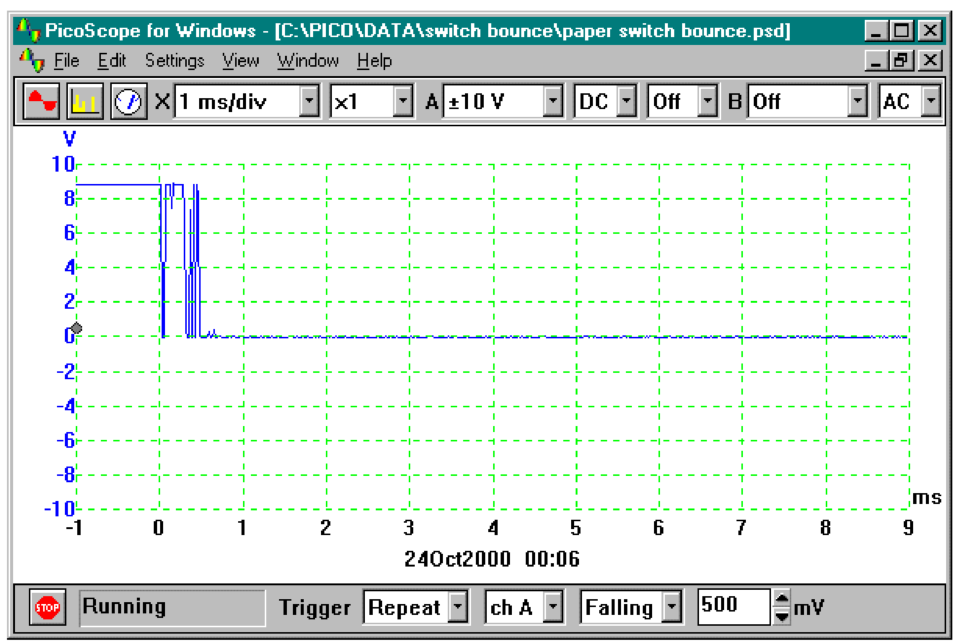
\includegraphics[width=0.65\textwidth]{Figures/debounce-handout-time-graph.pdf}
	\caption{A Bouncing Input Signal from a Switch}
	\label{debounce-handout-time-graph}
\end{figure}

From Professor Vemuri's lecture,
\hyperref[debounce-handout-time-graph]{figure \ref{debounce-handout-time-graph}}
shows the timescale at which some random switch bounces.
Based on this plot, the expected bouncing time of \texttt{SW1}
was on the order of $500\, \mu s$.

\section{Experiment and Design Revisions}

\subsection{Command Line Assembly}

My \texttt{.asm} source files were assembled on the command line so
please do this if they don't compile nicely in the IDE.
On Ubuntu, with the default MPLAB installation location, 
from the directory containting \texttt{catch-the-clown.asm}, the commands are:
\begin{verbatim}
$ cp /opt/microchip/mplabx/v3.10/mpasmx/p16f887.inc ./p16f887.inc
$ /opt/microchip/mplabx/v3.10/mpasmx/mpasmx -p16f887 catch-the-clown.asm
$ more catch-the-clown.ERR
\end{verbatim}

\subsection{PORTB Input}

On the 44--pin demo board, the pushbutton is connected to \texttt{RB0}
on \texttt{PORTB}, in an active low configuration with a $1k\Omega$, $10k\Omega$
voltage divider, as shown in \hyperref[io-circuit-diagram]{figure \ref{io-circuit-diagram}}.

When I first wrote my implementation for part 1 of the lab,
I could not get the $\mu$Controller to respond to pressing the
pushbutton switch (SW1). After inspecting the hardware with a ohmmeter,
I knew the problem had to be in software. I created a knew `hello world'
program for debugging the pushbutton switch.

It turns out the bug was a configuration problem: \texttt{RB0} is connected
to one of the 16 analog inputs, \texttt{AD12}. By default, the pin configured
use with the ADC and the digital input amplifiers are turned off.
Here is a nugget that was buried on page 49 of the PIC16F887 datasheet:
\begin{center}
	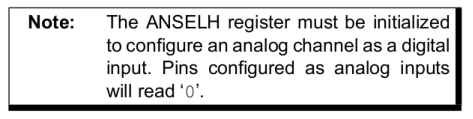
\includegraphics[width=0.5\textwidth]{Figures/port-b-configuration-note.pdf}
	\captionof{figure}{Port B Configuration Note}
\end{center}
With this nugget, the working `pushbutton hello world' program was:
\lstinputlisting[backgroundcolor=\color{mygray}, basicstyle=\small]{Test-SW1/test-sw1.asm}

\subsection{Adjusting Debounce Time}

The results from part 1 of the lab are presented in
hyperref[part-1-results-section]{section \ref{part-1-results-section}}.
From these results, the \texttt{DEBOUNCE\_TIME} for the part 2 implementation
was adjusted to XXX to require a steady state, debouncing period of
\begin{equation*}
T=X*14\, \mu s=XXX
\end{equation*}
before a switch activation is accepted by the program.

\section{Observations}

\subsection{44--Pin Demo Board \texttt{SW1} Bouncing Time}
\label{part-1-results-section}

\section{Discussion}

\clearpage

\section{Implementation Code}

\subsection{Does the Switch Bounce?}
\label{debounce-time-code}
\lstinputlisting[breaklines, basicstyle=\small]{Debounce-Time/debounce-time.asm}

\clearpage
\subsection{Catch the Clown!}
\label{catch-the-clown-code}
\lstinputlisting[breaklines, basicstyle=\small]{Catch-the-Clown/catch-the-clown.asm}

\end{document}
